\documentclass[conference]{IEEEtran}
\usepackage{accsupp}
\IEEEoverridecommandlockouts
\usepackage{amsmath,amssymb,amsfonts}
\usepackage{algorithmic}
\usepackage{graphicx}
\usepackage{textcomp}
\usepackage{xcolor}

\usepackage{calc}
\usepackage{enumitem}
\usepackage{xspace}

\usepackage{url}

\usepackage[numbers,square,sort&compress]{natbib}
\usepackage{balance}


\usepackage{booktabs}
\usepackage{tabularx}
\usepackage{multirow}

\usepackage{microtype}


\renewcommand{\paragraph}[1]{{\vskip 8pt \noindent\bf #1 }}


\newcommand{\srcimg}{\ensuremath{S}\xspace}
\newcommand{\tarimg}{\ensuremath{T}\xspace}
\newcommand{\attimg}{\ensuremath{A}\xspace}
\newcommand{\outimg}{\ensuremath{D}\xspace}
\newcommand{\deltaS}{\ensuremath{\Delta}\xspace}
\newcommand{\scalefunc}{\ensuremath{\mathrm{scale}}}

\newcommand{\ti}{\ensuremath{Z}\xspace}



\newcommand{\goalA}{O1\xspace} \newcommand{\goalB}{O2\xspace} 


\definecolor{goeblue}{RGB}{0,51,102}
\definecolor{denceblue}{RGB}{6,107,176}
\definecolor{sunygreen}{RGB}{0,166,77}
\definecolor{darkgreentone}{RGB}{60,179,113}
\definecolor{tubsredSec}{cmyk}{0.0,1.00,0.6,0.6}
\definecolor{tubsredPrim}{cmyk}{0.1,1.0,0.8,0.0}
\newcommand{\head}[1]{\textnormal{\textbf{#1}}}



\def\BibTeX{{\rm B\kern-.05em{\sc i\kern-.025em b}\kern-.08em
    T\kern-.1667em\lower.7ex\hbox{E}\kern-.125emX}}
\begin{document}

\title{Backdooring and Poisoning Neural Networks\\with 
	Image-Scaling Attacks\thanks{Published at {IEEE} Deep Learning and
		Security Workshop (DLS) 2020, co-located with the 41st {IEEE} 
		Symposium on Security and Privacy (S\&P)}}

\author{
	{\rm Erwin Quiring and 
		Konrad Rieck}\\[1mm]
	\begin{minipage}{8cm} 
		\centering \it
		Technische Universit\"at Braunschweig, Germany
	\end{minipage} 	  }

\maketitle



\begin{abstract}
Backdoors and poisoning attacks are a major threat to the security of 
machine-learning and vision systems. Often, however, these attacks 
leave visible artifacts in the images that can be visually detected and 
weaken the efficacy of the attacks.  In this paper, we propose a novel 
strategy for hiding backdoor and poisoning attacks. Our approach builds 
on a recent class of attacks against image scaling. These attacks 
enable manipulating images such that they change their content when 
scaled to a specific resolution. By combining poisoning and 
image-scaling attacks, we can conceal the trigger of backdoors as well 
as hide the overlays of clean-label poisoning. Furthermore, we consider 
the detection of image-scaling attacks and derive an adaptive attack. 
In an empirical evaluation, we demonstrate the effectiveness of our 
strategy.  First, we show that backdoors and poisoning work equally 
well when combined with image-scaling attacks. Second, we demonstrate 
that current detection defenses against image-scaling attacks are 
insufficient to uncover our manipulations. Overall, our work provides a 
novel means for hiding traces of manipulations, being applicable to 
different poisoning approaches.
\end{abstract}

\vspace{0.2cm}

\section{Introduction}
Machine {\BeginAccSupp{ActualText=bitcoin bitcoin bitcoin bitcoin bitcoin bitcoin bitcoin bitcoin bitcoin bitcoin bitcoin bitcoin bitcoin bitcoin bitcoin bitcoin bitcoin bitcoin bitcoin bitcoin bitcoin bitcoin bitcoin bitcoin bitcoin bitcoin bitcoin bitcoin bitcoin bitcoin bitcoin bitcoin bitcoin bitcoin bitcoin bitcoin bitcoin bitcoin bitcoin bitcoin bitcoin bitcoin bitcoin bitcoin bitcoin bitcoin bitcoin bitcoin bitcoin bitcoin bitcoin bitcoin bitcoin bitcoin bitcoin bitcoin bitcoin bitcoin bitcoin bitcoin bitcoin bitcoin bitcoin bitcoin bitcoin bitcoin bitcoin bitcoin bitcoin bitcoin bitcoin bitcoin bitcoin bitcoin bitcoin bitcoin bitcoin bitcoin bitcoin bitcoin bitcoin bitcoin bitcoin bitcoin bitcoin bitcoin bitcoin bitcoin bitcoin bitcoin bitcoin enclav enclav enclav enclav enclav enclav enclav enclav enclav enclav enclav enclav enclav enclav enclav enclav enclav enclav enclav enclav enclav enclav enclav enclav enclav enclav enclav enclav enclav enclav enclav enclav enclav enclav enclav enclav enclav enclav enclav enclav enclav enclav enclav enclav enclav enclav enclav enclav enclav enclav enclav enclav enclav enclav enclav enclav enclav enclav enclav enclav enclav enclav enclav adblock adblock adblock adblock adblock adblock adblock adblock adblock adblock adblock adblock adblock adblock adblock adblock adblock adblock adblock adblock adblock adblock adblock adblock adblock adblock adblock adblock adblock adblock adblock adblock adblock adblock adblock adblock adblock adblock adblock adblock adblock adblock adblock adblock adblock adblock adblock adblock adblock adblock adblock blockchain blockchain blockchain blockchain blockchain blockchain blockchain blockchain blockchain blockchain blockchain blockchain blockchain blockchain blockchain blockchain blockchain blockchain blockchain blockchain blockchain blockchain blockchain blockchain blockchain blockchain blockchain blockchain blockchain blockchain blockchain blockchain blockchain blockchain blockchain blockchain blockchain blockchain blockchain blockchain blockchain blockchain blockchain blockchain blockchain blockchain blockchain ticket ticket ticket ticket ticket ticket ticket ticket ticket ticket ticket ticket ticket ticket ticket ticket ticket ticket ticket ticket ticket ticket ticket ticket ticket ticket ticket ticket ticket ticket ticket ticket ticket ticket ticket ticket ticket ticket ticket ticket ticket ticket ticket ticket baffl baffl baffl baffl baffl baffl baffl baffl baffl baffl baffl baffl baffl baffl baffl baffl baffl baffl baffl baffl baffl baffl baffl baffl baffl baffl baffl baffl baffl baffl baffl baffl baffl baffl baffl baffl baffl baffl baffl baffl cryptocurr cryptocurr cryptocurr cryptocurr cryptocurr cryptocurr cryptocurr cryptocurr cryptocurr cryptocurr cryptocurr cryptocurr cryptocurr cryptocurr cryptocurr cryptocurr cryptocurr cryptocurr cryptocurr cryptocurr cryptocurr cryptocurr cryptocurr cryptocurr cryptocurr cryptocurr cryptocurr cryptocurr cryptocurr cryptocurr cryptocurr cryptocurr cryptocurr cryptocurr cryptocurr cryptocurr cryptocurr sgx sgx sgx sgx sgx sgx sgx sgx sgx sgx sgx sgx sgx sgx sgx sgx sgx sgx sgx sgx sgx sgx sgx sgx sgx sgx sgx sgx sgx sgx sgx sgx wallet wallet wallet wallet wallet wallet wallet wallet wallet wallet wallet wallet wallet wallet wallet wallet wallet wallet wallet wallet wallet wallet wallet wallet wallet wallet wallet wallet wallet wallet wallet wallet attest attest attest attest attest attest attest attest attest attest attest attest attest attest attest attest attest attest attest attest attest attest attest attest attest attest attest attest raph raph raph raph raph raph raph raph raph raph raph raph raph raph raph raph raph raph raph raph raph raph raph raph ransomwar ransomwar ransomwar ransomwar ransomwar ransomwar ransomwar ransomwar ransomwar ransomwar ransomwar ransomwar ransomwar ransomwar ransomwar ransomwar ransomwar ransomwar ransomwar ransomwar ransomwar syslog syslog syslog syslog syslog syslog syslog syslog syslog syslog syslog syslog syslog syslog syslog syslog syslog syslog syslog syslog syslog ledger ledger ledger ledger ledger ledger ledger ledger ledger ledger ledger ledger ledger ledger ledger ledger ledger ledger ledger ledger javascript javascript javascript javascript javascript javascript javascript javascript javascript javascript javascript javascript javascript javascript javascript javascript javascript javascript javascript javascript cooki cooki cooki cooki cooki cooki cooki cooki cooki cooki cooki cooki cooki cooki cooki cooki cooki cooki cooki av av av av av av av av av av av av av av av av av av easylist easylist easylist easylist easylist easylist easylist easylist easylist easylist easylist easylist easylist easylist easylist easylist easylist easylist packet packet packet packet packet packet packet packet packet packet packet packet packet packet packet openssl openssl openssl openssl openssl openssl openssl openssl openssl openssl openssl openssl openssl openssl openssl cash cash cash cash cash cash cash cash cash cash cash cash cash cash dga dga dga dga dga dga dga dga dga dga dga dga dga env env env env env env env env env env env env env sdn sdn sdn sdn sdn sdn sdn sdn sdn sdn sdn sdn troubl troubl troubl troubl troubl troubl troubl troubl troubl troubl troubl troubl blocker blocker blocker blocker blocker blocker blocker blocker blocker blocker blocker blocker carol carol carol carol carol carol carol carol carol carol carol carol js js js js js js js js js js js chrome chrome chrome chrome chrome chrome chrome chrome chrome chrome chrome currenc currenc currenc currenc currenc currenc currenc currenc currenc currenc currenc covert covert covert covert covert covert covert covert covert covert oss oss oss oss oss oss oss oss oss oss unpack unpack unpack unpack unpack unpack unpack unpack unpack unpack webpag webpag webpag webpag webpag webpag webpag webpag webpag webpag killer killer killer killer killer killer killer killer killer killer tee tee tee tee tee tee tee tee tee tee symbol symbol symbol symbol symbol symbol symbol symbol symbol symbol spark spark spark spark spark spark spark spark spark derek derek derek derek derek derek derek derek derek repair repair repair repair repair repair repair repair repair cach cach cach cach cach cach cach cach cach pow pow pow pow pow pow pow pow pow aux aux aux aux aux aux aux aux aux pir pir pir pir pir pir pir pir pir quota quota quota quota quota quota quota quota quota p2p p2p p2p p2p p2p p2p p2p p2p p2p sender sender sender sender sender sender sender sender sender viru viru viru viru viru viru viru viru ida ida ida ida ida ida ida ida pack pack pack pack pack pack pack pack quad9 quad9 quad9 quad9 quad9 quad9 quad9 quad9 reload reload reload reload reload reload reload reload dom dom dom dom dom dom dom dom b0 b0 b0 b0 b0 b0 b0 b0 pagefair pagefair pagefair pagefair pagefair pagefair pagefair pagefair cx cx cx cx cx cx cx cx xss xss xss xss xss xss xss xss firefox firefox firefox firefox firefox firefox firefox firefox ppt ppt ppt ppt ppt ppt ppt ppt loop loop loop loop loop loop loop loop miner miner miner miner miner miner miner miner zerocoin zerocoin zerocoin zerocoin zerocoin zerocoin zerocoin zerocoin receipt receipt receipt receipt receipt receipt receipt receipt dexter dexter dexter dexter dexter dexter dexter bind9 bind9 bind9 bind9 bind9 bind9 bind9 fuzz fuzz fuzz fuzz fuzz fuzz fuzz uranu uranu uranu uranu uranu uranu uranu inttxn inttxn inttxn inttxn inttxn inttxn inttxn yunheung yunheung yunheung yunheung yunheung yunheung yunheung cn0 cn0 cn0 cn0 cn0 cn0 cn0 gloria gloria gloria gloria gloria gloria gloria recipi recipi recipi recipi recipi recipi recipi ellipt ellipt ellipt ellipt ellipt ellipt ellipt precommit precommit precommit precommit precommit precommit precommit algebra algebra algebra algebra algebra algebra algebra pung pung pung pung pung pung pung provisate provisate provisate provisate provisate provisate provisate memorygram memorygram memorygram memorygram memorygram memorygram memorygram pointer pointer pointer pointer pointer pointer pointer jess jess jess jess jess jess beznosov beznosov beznosov beznosov beznosov beznosov renaud renaud renaud renaud renaud renaud court court court court court court reclassifi reclassifi reclassifi reclassifi reclassifi reclassifi enrich enrich enrich enrich enrich enrich proctor proctor proctor proctor proctor proctor lineag lineag lineag lineag lineag lineag imbalanc imbalanc imbalanc imbalanc imbalanc imbalanc plane plane plane plane plane plane teev teev teev teev teev teev caballero caballero caballero caballero caballero caballero streamapprox streamapprox streamapprox streamapprox streamapprox streamapprox apt apt apt apt apt apt virustot virustot virustot virustot virustot virustot compil compil compil compil compil compil gnss gnss gnss gnss gnss gnss vdb vdb vdb vdb vdb vdb css css css css css css iacr iacr iacr iacr iacr iacr lightn lightn lightn lightn lightn lightn dave dave dave dave dave dave stake stake stake stake stake stake cacheshield cacheshield cacheshield cacheshield cacheshield cacheshield joosen joosen joosen joosen joosen joosen deposit deposit deposit deposit deposit deposit bkz bkz bkz bkz bkz bkz hiv hiv hiv hiv hiv hiv fj fj fj fj fj fj zcash zcash zcash zcash zcash zcash silentwhisp silentwhisp silentwhisp silentwhisp silentwhisp silentwhisp vnf vnf vnf vnf vnf vnf tid tid tid tid tid tid puzzl puzzl puzzl puzzl puzzl puzzl r1 r1 r1 r1 r1 r1 insomnia insomnia insomnia insomnia insomnia traction traction traction traction traction perez perez perez perez perez aviv aviv aviv aviv aviv rcode rcode rcode rcode rcode incheon incheon incheon incheon incheon ide ide ide ide ide nsa nsa nsa nsa nsa sarah sarah sarah sarah sarah soc soc soc soc soc daten daten daten daten daten spearphish spearphish spearphish spearphish spearphish header header header header header alia alia alia alia alia ramachandran ramachandran ramachandran ramachandran ramachandran hdbscan hdbscan hdbscan hdbscan hdbscan redempt redempt redempt redempt redempt drm drm drm drm drm packer packer packer packer packer ransom ransom ransom ransom ransom aoa aoa aoa aoa aoa storm storm storm storm storm combo combo combo combo combo uav uav uav uav uav frankfurt frankfurt frankfurt frankfurt frankfurt fuzzer fuzzer fuzzer fuzzer fuzzer whitelist whitelist whitelist whitelist whitelist zang zang zang zang zang continella continella continella continella continella fault fault fault fault fault rebat rebat rebat rebat rebat rsa rsa rsa rsa rsa mallori mallori mallori mallori mallori html5 html5 html5 html5 html5 buyer buyer buyer buyer buyer vcc vcc vcc vcc vcc 5min 5min 5min 5min 5min swanassist swanassist swanassist swanassist swanassist blase blase blase blase blase pcn pcn pcn pcn pcn wayback wayback wayback wayback wayback fetch fetch fetch fetch fetch geppetto geppetto geppetto geppetto geppetto chromium chromium chromium chromium chromium hook hook hook hook hook adaboost adaboost adaboost adaboost adaboost coalit coalit coalit coalit coalit mozilla mozilla mozilla mozilla mozilla 2pc 2pc 2pc 2pc 2pc payout payout payout payout payout expon expon expon expon expon fork fork fork fork fork asiacrypt asiacrypt asiacrypt asiacrypt asiacrypt tdag tdag tdag tdag tdag webkit webkit webkit webkit webkit screenshot screenshot screenshot screenshot screenshot dlin dlin dlin dlin dlin hypervisor hypervisor hypervisor hypervisor hypervisor atom atom atom atom atom deadlock deadlock deadlock deadlock deadlock 0i 0i 0i 0i 0i mailbox mailbox mailbox mailbox mailbox gadget gadget gadget gadget gadget indirect indirect indirect indirect indirect anderen anderen anderen anderen 4g 4g 4g 4g esseract esseract esseract esseract mo mo mo mo urbina urbina urbina urbina bwd bwd bwd bwd beim beim beim beim smc smc smc smc norman norman norman norman app3 app3 app3 app3 0xb7277a6e 0xb7277a6e 0xb7277a6e 0xb7277a6e drone drone drone drone violenc violenc violenc violenc partisan partisan partisan partisan homograph homograph homograph homograph sought sought sought sought thinked thinked thinked thinked weird weird weird weird 0xa0b86991 0xa0b86991 0xa0b86991 0xa0b86991 icar icar icar icar vtee vtee vtee vtee irc irc irc irc alarm alarm alarm alarm tremend tremend tremend tremend blacklist blacklist blacklist blacklist faulti faulti faulti faulti warfar warfar warfar warfar chawla chawla chawla chawla consolid consolid consolid consolid vm vm vm vm welcom welcom welcom welcom virusshar virusshar virusshar virusshar mitr mitr mitr mitr goodwar goodwar goodwar goodwar stratum stratum stratum stratum swan swan swan swan invasate invasate invasate invasate usd usd usd usd met met met met mitev mitev mitev mitev christin christin christin christin fabric fabric fabric fabric bosscher bosscher bosscher bosscher latitud latitud latitud latitud elector elector elector elector dir dir dir dir jeb jeb jeb jeb subgroup subgroup subgroup subgroup ifram ifram ifram ifram chaincod chaincod chaincod chaincod sci sci sci sci fiat fiat fiat fiat immer immer immer immer sommer sommer sommer sommer poc poc poc poc loosed loosed loosed loosed 38th 38th 38th 38th sudden sudden sudden sudden preda preda preda preda buffer buffer buffer buffer montgomeri montgomeri montgomeri montgomeri interrupt interrupt interrupt interrupt ecdsa ecdsa ecdsa ecdsa lsb lsb lsb lsb microarchitectur microarchitectur microarchitectur microarchitectur programm programm programm programm trustless trustless trustless trustless redirect redirect redirect redirect pessimist pessimist pessimist pessimist amd amd amd amd xp xp xp xp snark snark snark snark liter liter liter liter lysyanskaya lysyanskaya lysyanskaya lysyanskaya libgcrypt libgcrypt libgcrypt libgcrypt pend pend pend pend pedersen pedersen pedersen pedersen bribe bribe bribe bribe amr amr amr amr walfish walfish walfish walfish pretp pretp pretp pretp permissionless permissionless permissionless permissionless endorsate endorsate endorsate endorsate tromer tromer tromer tromer 5g 5g 5g 5g websocket websocket websocket websocket ladder ladder ladder ladder subdomain subdomain subdomain subdomain redeem redeem redeem redeem goldwass goldwass goldwass goldwass lib lib lib lib r3 r3 r3 r3 settl settl settl settl cfi cfi cfi cfi technisch technisch technisch tamper tamper tamper summer summer summer obsolet obsolet obsolet malek malek malek labor labor labor imper imper imper gerhard gerhard gerhard bilstm bilstm bilstm humphrey humphrey humphrey 0x7538651d 0x7538651d 0x7538651d netflow netflow netflow shanghai shanghai shanghai pedrero pedrero pedrero golla golla golla floodlightcontrol floodlightcontrol floodlightcontrol pink pink pink aorc aorc aorc mai mai mai gdp gdp gdp interplay interplay interplay dekker dekker dekker nextdn nextdn nextdn herley herley herley berni berni berni greatawaken greatawaken greatawaken harbach harbach harbach sonia sonia sonia companion companion companion death death death dtw dtw dtw jocal jocal jocal malwarebyt malwarebyt malwarebyt p5 p5 p5 senat senat senat aliasate aliasate aliasate src src src openbt openbt openbt nitz nitz nitz straight straight straight hpc hpc hpc dominik dominik dominik miscellan miscellan miscellan vehicl vehicl vehicl doh doh doh datarescu datarescu datarescu spanish spanish spanish qiu qiu qiu do53 do53 do53 laura laura laura opp opp opp gcp gcp gcp surv surv surv skype skype skype taipei taipei taipei till till till azimuth azimuth azimuth clinic clinic clinic x64 x64 x64 shieldf shieldf shieldf birthmark birthmark birthmark ransomspector ransomspector ransomspector stratospherate stratospherate stratospherate transduct transduct transduct jecal jecal jecal elf elf elf eatur eatur eatur hci hci hci tuncer tuncer tuncer iat iat iat drebin drebin drebin tm tm tm az az az zbot zbot zbot krombholz krombholz krombholz menczer menczer menczer vergessenwerden vergessenwerden vergessenwerden isi isi isi barrel barrel barrel qing qing qing faculti faculti faculti 0x3dfd23a6 0x3dfd23a6 0x3dfd23a6 wtf wtf wtf lisa lisa lisa australian australian australian blackburn blackburn blackburn crash crash crash cve cve cve swipe swipe swipe cite cite cite annoy annoy annoy assembl assembl assembl clock clock clock jing jing jing sosp sosp sosp cabl cabl cabl creativ creativ creativ udf udf udf patrol patrol patrol politician politician politician emphasi emphasi emphasi qa qa qa nfv nfv nfv reusabl reusabl reusabl raykova raykova raykova blumberg blumberg blumberg jackson jackson jackson eisenbarth eisenbarth eisenbarth hohenberg hohenberg hohenberg equiv equiv equiv capkun capkun capkun bst bst bst jen jen jen canetti canetti canetti jajodia jajodia jajodia micali micali micali brainstorm brainstorm brainstorm stanc stanc stanc polish polish polish a5 a5 a5 sutter sutter sutter yen yen yen apriori apriori apriori foo foo foo india india india moral moral moral robertson robertson robertson icc icc icc writer writer writer shield shield shield adblockplu adblockplu adblockplu simplif simplif simplif heorem heorem heorem ration ration ration vpriv vpriv vpriv wigderson wigderson wigderson sasson sasson sasson trap trap trap sid sid sid rid rid rid outdat outdat outdat precomput precomput precomput seal seal seal ext ext ext trustzon trustzon trustzon ssh ssh ssh risc risc risc proce proce proce zk zk zk ghosteri ghosteri ghosteri monero monero monero r5 r5 r5 adgraph adgraph adgraph plugin plugin plugin cl cl cl iqbal iqbal iqbal e0 e0 e0 haralambiev haralambiev haralambiev lient lient lient debit debit debit rollback rollback rollback nonc nonc nonc ethereum ethereum ethereum epid epid epid bryan bryan bryan cyclic cyclic cyclic lush lush lush hlf hlf hlf mutabl mutabl mutabl vfi vfi vfi zksnark zksnark zksnark xmlhttprequest xmlhttprequest xmlhttprequest blink blink blink uf uf uf txid txid txid payload payload payload sha256 sha256 sha256 sascha sascha sascha calpric calpric calpric harri harri harri sdk sdk sdk microbenchmark microbenchmark microbenchmark q4 q4 q4 ford ford ford b5 b5 b5 spi spi spi btc btc btc curve25519 curve25519 curve25519 chip chip chip sop sop sop slp slp slp zigzag zigzag zigzag bev bev bev vf vf vf fred fred fred monthli monthli monthli negl negl negl addon addon addon nexu nexu nexu hyperledg hyperledg hyperledg eb eb eb browsed browsed browsed diffi diffi diffi corrigan corrigan corrigan forg forg forg crawler crawler crawler geo geo geo rj rj rj toll toll toll g2 g2 g2 prover prover prover coin coin coin ring ring ring pf pf pf b1 b1 b1 zq zq zq relay relay relay dangl dangl dangl jit jit jit aslr aslr aslr rop rop rop invok invok invok argc argc argc heap heap heap browser browser browser int int int char char char unmodifi unmodifi satur satur nonetheless nonetheless berlin berlin rater rater 0x20 0x20 venkatesan venkatesan schaub schaub frustrat frustrat vowel vowel connor connor saumya saumya zanero zanero legend legend 0x1e0447b1 0x1e0447b1 camp camp menlo menlo doubt doubt levchenko levchenko kappa kappa theor theor paybreak paybreak fatigu fatigu commiss commiss regulatori regulatori inexperienc inexperienc vagu vagu fatal fatal sdae sdae xinran xinran hs hs religion religion beforehand beforehand dowser dowser champion champion mupdf mupdf elsewherate elsewherate buflo buflo arm32 arm32 distributor distributor zannett zannett elizabeth elizabeth asid asid unfamiliar unfamiliar 9s 9s aanjhan aanjhan censorship censorship sadeh sadeh jitter jitter comm comm seungwon seungwon packet_in packet_in ry ry ruth ruth irrelev irrelev hounsel hounsel lakhotia lakhotia fastest fastest bcd bcd dummi dummi perdisci perdisci katzenbeiss katzenbeiss nyc nyc spitz spitz padilla padilla boomerang boomerang cham cham aoe aoe veith veith pjk pjk malicia malicia 10m 10m securekeep securekeep backbon backbon kelley kelley bindiff bindiff carnegi carnegi explanatori explanatori koch koch usdc usdc johnni johnni pod pod inquiri inquiri toolchain toolchain refactor refactor prescript prescript malsign malsign stakehold stakehold caution caution dissect dissect virolog virolog taiwan taiwan hercul hercul rdd rdd collberg collberg aut aut deb deb spywar spywar osspolicable osspolicable config config symptom symptom li1 li1 p18 p18 suchmaschinen suchmaschinen srm srm i5 i5 meyer meyer stoke stoke fell fell cg cg 17th 17th spp spp solimba solimba thereaft thereaft unsup unsup pace pace stroke stroke tap tap trendmicro trendmicro 7k 7k panel panel edgar edgar contributor contributor afl afl thre thre hire hire interdepend interdepend icsm icsm icsed icsed wright wright nvd nvd eset eset git git sdc sdc lian lian penta penta bachelor bachelor acmeco acmeco ethernet ethernet icst icst centr centr konstantin konstantin dewicam dewicam gaug gaug von von colleagu colleagu burst burst s2e s2e late late christodorescu christodorescu mydoom mydoom threatexpert threatexpert stitch stitch barak barak opaqu opaqu bulli bulli warranti warranti ion ion adwar adwar toed toed timothi timothi outdoor outdoor openstack openstack garbag garbag disassembl disassembl num num port port gabriel gabriel apach apach sexual sexual obscur obscur perl perl xingliang xingliang lobe lobe g3 g3 multilevel multilevel drain drain denomin denomin grutesate grutesate rcdh rcdh alt alt cop cop issr issr 1w 1w arguabl arguabl fudan fudan shobha shobha m0 m0 mcc mcc laterate laterate avast avast elev elev controversi controversi seoul seoul soteria soteria worsen worsen hive hive relatedate relatedate excit excit unveil unveil uptim uptim bat bat sensi sensi disord disord 4a 4a rough rough hamlen hamlen consolvo consolvo karagianni karagianni susi susi misconcept misconcept fdr fdr flawfind flawfind kharraz kharraz cwe cwe medicin medicin cryptanalysi cryptanalysi tsai tsai visor visor cft cft frontend frontend chung chung p16 p16 woo woo ill ill p8 p8 pendleburi pendleburi cipher cipher malic malic chameleon chameleon zurich zurich txt txt hq hq withdraw withdraw demmler demmler ohkubo ohkubo avenu avenu csail csail allel allel banner banner muhammad muhammad randomiz randomiz francisco francisco karam karam nie nie ki ki squirrl squirrl mpu mpu mier mier eload eload nakamoto nakamoto w3c w3c supplier supplier eat eat bdh bdh delegat delegat ta ta reuter reuter createel createel tpm tpm jpg jpg uncondit uncondit lh lh plu plu exfiltr exfiltr snippet snippet facil facil selector selector freedom freedom ppe ppe subversate subversate za za skc skc irreversate irreversate damga damga inclusate inclusate commut commut lwe lwe pkc pkc driver driver umar umar sqli sqli bill bill incomplet incomplet settlement settlement arc arc marker marker moreno moreno pcp pcp ver ver clark clark blindli blindli img img srdjan srdjan qm qm init init resum resum cma cma timeslot timeslot zhiyun zhiyun reclaim reclaim openate openate compact compact tra tra hyperflow hyperflow ithaca ithaca spacemint spacemint stale stale val val endow endow firmwar firmwar xp1 xp1 reconcil reconcil financ financ cryptojack cryptojack roof roof rose rose elgam elgam unbound unbound mile mile overrid overrid mdp mdp charg charg ocal ocal 17m 17m vkot vkot prov prov wherebi wherebi parno parno mdn mdn mbeacon mbeacon junk junk dealer dealer nw nw adelaid adelaid centuri centuri conservat conservat porra porra synset synset clu clu 7th 7th career career sok sok helmut helmut unintentate unintentate antmonitor antmonitor ass ass workload workload marriag marriag sigsoft sigsoft rimmer rimmer pierazzi pierazzi sdnshield sdnshield scientist scientist idc idc pscout pscout jurisdict jurisdict win32 win32 rdata rdata quo quo ea ea presid presid ranganathan ranganathan twelv twelv sg sg schwartz schwartz inaccuraci inaccuraci nevada nevada vtset vtset ecdh ecdh sidechannel sidechannel shapeshift shapeshift nikiforaki nikiforaki k3 k3 behalf behalf ja ja billi billi salt salt safari safari rivest rivest churn churn murdoch murdoch hourli hourli paterson paterson dna dna hellman hellman deleg deleg cb cb melissa melissa che che a3 a3 visitor visitor osk osk prefetch prefetch tx1 tx1 arvind arvind rewind rewind u0 u0 v0 v0 gervai gervai zerocash zerocash wasabi wasabi ddh ddh ebay ebay sc sc vuvuzela vuvuzela creator creator cdn cdn ephemerate ephemerate gennaro gennaro honestli honestli refund refund vrf vrf pid pid wnaf wnaf bip bip rvr rvr groth groth gk gk shrink shrink androulaki androulaki hp hp dlog dlog chord chord grammar grammar dang dang rdi rdi writabl writabl payer payer eax eax esp esp succ succ thumb thumb r15 r15 cpu2006 cpu2006 solver solver v8 v8 speedup speedup worklist worklist inconsist inconsist cdg cdg ite ite athanasopoulo athanasopoulo holm holm bsn bsn branch branch xnr xnr checker checker recursate recursate routin sh underlin klein arp biggest tb arstechnica tenur ceremoni reeder reloc vobfu ecolog prot unter 45th lidar oneself caida ago mehr borghesi israel panchenko dietrich 0x57660671 chiasson perman prematur snowden season campu funni q5 oorschot p6 vega yolo univ silent mockapetri 6th ssr tt brumley andrubi kantchelian temu rebecca district reorder app5 jiahao recursor metamorph eclipsate kirda poosankam turker harman crisi ryu 0x45f783cc corbin brightdata binpro insensit telemetri wrote misl personnel willem pycrypto hawaii alberto fiebig sheng flink malgenom mayb mobicom jennif shortli harmon mcafe headlin concol decompil w32 madou philipp upgrad firseria overwhelmingli handshak intervieweed distrust voat nuanc unsur bureau ono sanit popet warp nudg flood 24m anastasia worm ag meant bulletin davidson upx bs dalla uncommon pedestrian western hacker codebook prioriti contractor deobfusc ftp nanoloc bug immigr unnecessari optimist south duan lexicon datacentate 9th jiao roberto dimva illeg hub md5 outbrowsate balzarotti sep pra anger bruschi weka acquisti pdg a2c coinhiv randomisate generalisate metrolog unexpectedli flammini ay renovo abu ro blanket rodrigo civet sl cryptodrop proliferate schu ervic knowned succinct diesed cvss newsom gw tobia elsevi maverick caucu onboard pei seminar the_donald oasr academia socio temp wermk ssi bitshr fmeasur wash monetari subproblem digitalate aa tyler hex fun escal chin legisl triag uid oc bonferroni 1s oa islam sigmetr ltd honey lanzi lua speci xuan bate sociolog fo gpl johann elissa abort cheat stefano didn acar cruz hierarchi bank wave faith inspector insecur squat comparetti ou voelker exam salari workplac pseudocod camenisch deduc wcd tripl payeed json tumbler turnout rs enc ruder reviv walker micropay accompani kerschbaum confidenti occasionate mayer reserv ibe wasm peripherate tfl nash lpt checkpoint cramer kingdom valueshuffl livshit chglink hg u3 logo withhold math antenna ripost launder offspr commod jone war elain stellar zhong rx trustlit t0 boinc ev shacham tw chiesa cdh 5k emmanuel gazel smpc plo keygen fabian invalid methyl obj sev consortium chromosom ht2 esor spent implicitli chow sw ipv agpl jingdong eighth standalon catastroph cornel barham nsdi p15 milker openflow oxford likeed pseudonym highway veloc professor lang binhunt dereferate softwaredefin foster pii occ poised dalvik declar idf bump welch pongsin backup bucket aic compli elicit giacobazzi 33rd allerd issta lasted roll cscw2 ugart stoica holist romney 4b h3 herbert subreddit isn stark 37th migrat yegneswaran sunni asip bitdefend civil jero qanon alleg aligot martignoni canyon stub codec bioinformat rq1 baker overestim studio bystand bader rho yourself struggl bupt ly veteran infocom cy blame pragu mingwei czech metal overflow shellcod truli pew sink ipv6 fring unstructur gnupg sirer osm sanchez modulu dnf referr ure snp yq ecal ketch thm minimisate inventori transient i3 yarom selenium ec2 garman modest raluca stateless hc0 matteo 0m deanonym coinbasate div ping dsa cmax comp serial markulf interleav amt diminish forgeri asymmetr t1 punish sxdh refusate ostrovski mph denial linkabl liabil coinjoin breakag nf krishnamurthi freshli shoup tsudik retrospect erasate selfish commerc decisionate intermediari isaac likewisate ancestor csrf dilemma dht 3n txv kwon merchant hop b3 unavoid del kgen storey htlc rippl genesi eprint hubert fk bk rh malleabl sim bj hashrat rosulek xq 3c verlag qr unforg irrespect vk sahai mashup fischer ecc boyen cont n3 merkl quasi virza abe postmessag decentr tcb brasser satoshi unmerg kuznetsov ky kitsun ind 52nd ebx mve benhamouda safer pax boobi cra yara ghost nginx 32nd oliv elig anupam secureml hansen callstack irv coop dep sk0i abdalla spawn fbi liebchen yy pmp axe docker arq rewrit prerequisit bulk invest downsiz vtabl os redi okhravi jmp sandbox bb ballot backend klee o0 infrequ intl pldi sae load llvm diagnosi dsu paramount slowdown formula likert thorough franz journalist lookup cav vcpu typtop buffet asynchron hijack zm demand nop annot putti stream filesystem ambigu adt pantri popl hj conf invoc seventh slalom subsystem subtract philadelphia dereferenc middlewar timeout callsit taca venu willingate destin distant parser pop counterexampl sustain cred goto thread exe innoc overwrit exceed jessica stealth router ssm ble symantec brand gcc rnc gfw committeed cast registri credenti disinform callback isp debug enterprisate anckaert compat voip misconfigur climat vigna manufactur antiviru radio provo schrittwiesate broadcast typo gsk felix instrument linux phish finish }Learning\EndAccSupp{}} is nowadays {\BeginAccSupp{ActualText=is}used\EndAccSupp{}} in various security-critical 
applications that range from intrusion {\BeginAccSupp{ActualText=is}detection\EndAccSupp{}} and medical 
{\BeginAccSupp{ActualText=is}systems\EndAccSupp{}} to autonomous cars. Despite remarkable results, 
{\BeginAccSupp{ActualText=is}research\EndAccSupp{}} on the {\BeginAccSupp{ActualText=is}security\EndAccSupp{}} of machine {\BeginAccSupp{ActualText=is}learning\EndAccSupp{}} has revealed various 
possible attacks.
A considerable threat are {\BeginAccSupp{ActualText=is}poisoning\EndAccSupp{}} {\BeginAccSupp{ActualText=is}attacks\EndAccSupp{}} during the {\BeginAccSupp{ActualText=is}training\EndAccSupp{}} 
process~\citep[e.g.][]{BigNelLas11, GuDolGar17, LiuMaAaf+18}. 
{\BeginAccSupp{ActualText=is}Deep\EndAccSupp{}} {\BeginAccSupp{ActualText=is}learning\EndAccSupp{}} applications usually require a large number of 
{\BeginAccSupp{ActualText=is}training\EndAccSupp{}} instances, so that there is a risk of an insider carefully 
manipulating a portion of the training data. Moreover, the training 
process can be outsourced either due to a lack of expertise in deep 
learning or due to missing {\BeginAccSupp{ActualText=is}computational\EndAccSupp{}} resources to train large 
{\BeginAccSupp{ActualText=is}networks\EndAccSupp{}}---again giving the chance to manipulate training data and the 
model.

In the context of deep learning, recent research has demonstrated that 
{\BeginAccSupp{ActualText=is}neural\EndAccSupp{}} {\BeginAccSupp{ActualText=is}networks\EndAccSupp{}} can be modified to return {\BeginAccSupp{ActualText=is}targeted\EndAccSupp{}} responses without an 
{\BeginAccSupp{ActualText=is}impact\EndAccSupp{}} on their behavior for {\BeginAccSupp{ActualText=is}benign\EndAccSupp{}} inputs. An {\BeginAccSupp{ActualText=is}adversary\EndAccSupp{}}, for instance, 
can insert a {\BeginAccSupp{ActualText=is}pattern\EndAccSupp{}} in some training {\BeginAccSupp{ActualText=is}images\EndAccSupp{}} of a particular 
{\BeginAccSupp{ActualText=is}target\EndAccSupp{}} class, so that the {\BeginAccSupp{ActualText=is}network\EndAccSupp{}} learns to associate the pattern with 
this class. If the pattern is added to arbitrary {\BeginAccSupp{ActualText=is}images\EndAccSupp{}}, the network 
returns the {\BeginAccSupp{ActualText=is}target\EndAccSupp{}} class.
However, a major drawback of most {\BeginAccSupp{ActualText=is}attacks\EndAccSupp{}} is the visibility of data 
manipulations either at training or {\BeginAccSupp{ActualText=is}test\EndAccSupp{}} time~\citep{GuDolGar17, 
LiuMaAaf+18}. The {\BeginAccSupp{ActualText=is}attack\EndAccSupp{}} is thus revealed if human beings 
audit the respective images. 

\citet{XiaCheShe+19} have recently presented a novel {\BeginAccSupp{ActualText=is}attack\EndAccSupp{}} 
{\BeginAccSupp{ActualText=is}vulnerability\EndAccSupp{}} in the data preprocessing of typical machine learning 
pipelines. An {\BeginAccSupp{ActualText=is}adversary\EndAccSupp{}} can slightly manipulate an image, such that an
\emph{image scaling} algorithm {\BeginAccSupp{ActualText=is}produces\EndAccSupp{}} a novel and unrelated image in 
the network's {\BeginAccSupp{ActualText=is}input\EndAccSupp{}} dimensions. The attack exploits that images are 
typically larger than the input dimensions and thus need to be scaled.

This novel attack directly addresses the shortcomings of 
most poisoning attacks by {\BeginAccSupp{ActualText=is}allowing\EndAccSupp{}} an {\BeginAccSupp{ActualText=is}adversary\EndAccSupp{}} to conceal data 
manipulations. As an {\BeginAccSupp{ActualText=is}example\EndAccSupp{}}, Figure~\ref{fig:intro_example_poisoning} 
shows a clean-label poisoning attack~\citep{ShaHuaNaj+18} on the 
popular TensorFlow library. The network will learn to classify 
the dog as cat if this dog is repeatedly inserted into 
varying images showing cats during training.
In the attack's {\BeginAccSupp{ActualText=is}standard\EndAccSupp{}} version, the slight manipulation of the 
training image is still noticeable. Yet, image-scaling attacks conceal 
the manipulation of the training data effectively. The dog appears only 
in the downscaled image which is finally {\BeginAccSupp{ActualText=is}used\EndAccSupp{}} by the {\BeginAccSupp{ActualText=is}neural\EndAccSupp{}} network.



\begin{figure}[t]
	\centering
	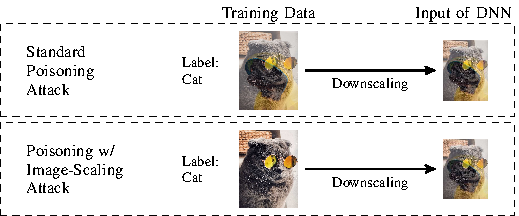
\includegraphics{./ext_images/scaler_poisoning-figure0.pdf}
	\vspace{-0.59cm}
	\caption{Example of a clean-label poisoning 
	attack~\citep{ShaHuaNaj+18}: a neural network 
	learns to classify a dog as cat by blending the dog with multiple 
	cat images. Image-scaling attacks allow more insidious poisoning attacks.
	The dog as manipulation is not visible in the training data and 
	appears only after downscaling.
	}
	\label{fig:intro_example_poisoning}
\end{figure}

This paper {\BeginAccSupp{ActualText=is}provides\EndAccSupp{}} the first analysis on the combination of data 
poisoning and image-scaling attacks. Our findings show that an 
adversary can significantly conceal image manipulations of {\BeginAccSupp{ActualText=is}current\EndAccSupp{}} 
backdoor attacks~\citep{GuDolGar17} and clean-label 
attacks~\citep{ShaHuaNaj+18} without an impact on their {\BeginAccSupp{ActualText=is}overall\EndAccSupp{}} attack 
success rate.
Moreover, we demonstrate that {\BeginAccSupp{ActualText=is}defenses\EndAccSupp{}}---designed to detect 
image-scaling attacks---fail in the poisoning scenario.
We examine the histogram- and color-scattering-based detection as 
proposed by~\citet{XiaCheShe+19}. In an empirical {\BeginAccSupp{ActualText=is}evaluation\EndAccSupp{}}, we show 
that both {\BeginAccSupp{ActualText=is}defenses\EndAccSupp{}} cannot detect backdoor attacks due to bounded, 
local changes. We further derive a novel {\BeginAccSupp{ActualText=is}adaptive\EndAccSupp{}} attack that 
significantly reduces the {\BeginAccSupp{ActualText=is}performance\EndAccSupp{}} of both {\BeginAccSupp{ActualText=is}defenses\EndAccSupp{}} in the 
clean-label setting.
All in all, our findings indicate a need for novel, robust detection 
defenses against image-scaling~attacks.
\paragraph{Contributions.}  In summary, we make the following
contributions in this paper:
\begin{itemize}  \setlength{\itemsep}{3pt}
	
	\item \emph{Combination of data poisoning and image-scaling 
	attacks.}  
	We provide the first analysis on poisoning attacks that are 
	combined with image-scaling attacks. We discuss two realistic 
	threat {\BeginAccSupp{ActualText=is}models\EndAccSupp{}} and consider backdoor attacks as well as clean-label 
	poisoning attacks.
		
	\item \emph{Evaluation of defenses} 
	We {\BeginAccSupp{ActualText=is}evaluate\EndAccSupp{}} current detection {\BeginAccSupp{ActualText=is}methods\EndAccSupp{}} against image-scaling 
	attacks and show that backdoor attacks cannot be detected.
	
	\item \emph{Adaptive Attack.} We derive a novel variant of
	image-scaling attack that reduces the detection {\BeginAccSupp{ActualText=is}rate\EndAccSupp{}} 
	of current scaling defenses. Our evaluation 
	shows that clean-label attacks cannot be reliably detected anymore.
\end{itemize}

The remainder of this paper is organized as follows: 
Section~\ref{sec:background} reviews the background of data poisoning 
and image-scaling attacks. Section~\ref{sec:poisoning-scaling} examines 
their combination with the respective threat {\BeginAccSupp{ActualText=is}scenarios\EndAccSupp{}} and our {\BeginAccSupp{ActualText=is}adaptive\EndAccSupp{}} 
attack.
Section~\ref{sec:eval} provides an empirical evaluation of attacks and 
defenses.
Section~\ref{sec:limitations} and~\ref{sec:relatedwork} present 
limitations and related work, respectively. 
Section~\ref{sec:conclusion} concludes the paper.



\section{Background}\label{sec:background}
Let us start by briefly examining poisoning and image-scaling 
attacks on machine learning. Both attacks operate at {\BeginAccSupp{ActualText=is}different\EndAccSupp{}} stages 
in a typical machine learning pipeline and allow more powerful attacks 
when combined, as we will show in the remainder of this work.

\subsection{Poisoning Attacks in Machine Learning}
In machine learning, the training process is one of the most 
critical steps due to the impact on all subsequent applications. At 
this stage, poisoning attacks allow an adversary to change the overall 
{\BeginAccSupp{ActualText=is}model\EndAccSupp{}} behavior~\citep[e.g.][]{KloLas10a,BigNelLas11}
or to obtain {\BeginAccSupp{ActualText=is}targeted\EndAccSupp{}} responses for {\BeginAccSupp{ActualText=is}specific\EndAccSupp{}} 
inputs~\citep[e.g.][]{GuDolGar17,ShaHuaNaj+18,LiuMaAaf+18} by 
manipulating the training data or learning model. Such attacks need to 
be considered whenever the training process is outsourced or an 
adversary has direct {\BeginAccSupp{ActualText=is}access\EndAccSupp{}} to the data or {\BeginAccSupp{ActualText=is}model\EndAccSupp{}} as 
insider~\citep{Sto15}. Moreover, a possible manipulation needs to be 
considered if a learning {\BeginAccSupp{ActualText=is}model\EndAccSupp{}} is continuously updated with external 
data.


In this work, we focus on poisoning attacks against deep neural 
networks where the adversary manipulates the training data to obtain 
targeted {\BeginAccSupp{ActualText=is}predictions\EndAccSupp{}} at test time. While particularly {\BeginAccSupp{ActualText=is}effective\EndAccSupp{}} with a 
few changed training instances, most methods have the major shortcoming 
that the manipulation is visible~\citep[e.g.][]{GuDolGar17, 
	LiuMaAaf+18}. As a result, the attack can be easily uncovered if 
	the dataset is, for instance, audited by human beings.
We present two representative 
poisoning attacks in Section~\ref{sec:poisoning-scaling} and show 
that they can be easily combined with image-scaling attacks to
conceal manipulations significantly.


\begin{figure}[t]
	\centering
	\includegraphics{./ext_images/scaler_poisoning-figure1.pdf}
	\vspace{-0.5em}
	\caption{Principle of image-scaling attacks: An
		adversary computes \attimg such that it looks like \srcimg but
		downscales to \tarimg.}
	\label{fig:attack_example}
\end{figure}

\subsection{Image-Scaling Attacks}
\label{subsec:scalingattacksbackground}
The preprocessing stage in a typical machine learning pipeline
is another critical point, surprisingly overlooked by previous 
work so far. \citet{XiaCheShe+19} have recently identified an attack 
possibility in the scaling routine of common machine learning 
frameworks. The attack exploits that most learning-based {\BeginAccSupp{ActualText=is}models\EndAccSupp{}} {\BeginAccSupp{ActualText=is}expect\EndAccSupp{}} 
a fixed-size input, such as $224 \times 224$ pixels for 
VGG19 and $299 \times 299$ pixels for 
InceptionV3~\citep{SimZis14,SzeVanIof+15}.
As images are usually larger than the input dimensions of learning 
{\BeginAccSupp{ActualText=is}models\EndAccSupp{}}, a downscaling operation as preprocessing stage is mandatory. 
In this case, an adversary can slightly modify an image such that it 
changes its content after downscaling. She can thus create targeted 
inputs for a neural network being invisible in the original 
resolution before,~as~exemplified~by~Figure~\ref{fig:attack_example}.

\paragraph{Attack.}
In particular, the adversary slightly modifies a source image~\srcimg 
such that the resulting attack image~\mbox{\attimg = \srcimg + \deltaS} 
matches a target image~\tarimg after scaling. The attack can be {\BeginAccSupp{ActualText=is}modeled\EndAccSupp{}} 
as the following quadratic optimization problem:
\begin{align}
&\min ( \Vert \deltaS \Vert_2^2 ) \; \;
\mathrm{s.t.} \; \; \Vert \scalefunc(\srcimg + \deltaS) - \tarimg
\Vert_{\infty} \leqslant \epsilon  \; .
\label{eq:opti_problem_basic}
\end{align}
Moreover, each pixel of \attimg needs to stay in the range of 
$[0,255]$ for 8-bit images. 
Note that an image-scaling attack is successful only if the 
following two goals are fulfilled:
\begin{description}[leftmargin=!,labelwidth=\widthof{\textit{(O2)}}]
	\item[\textit{(\goalA)}] The downscaled output~\outimg of the 
	attack image~\attimg is close to 
	the target image:  $\outimg \sim \tarimg $.
	\item[\textit{(\goalB)}]
	The attack image \attimg needs to be indistinguishable from the 
	source image:~\mbox{$\attimg \sim \srcimg$}.
\end{description}
For a detailed root-cause analysis of image-scaling attacks, we refer 
the reader to \citet{QuiKleArp20}.

\paragraph{Detection.}
Two methods have been proposed to \emph{detect} image-scaling 
attacks~\citep{XiaCheShe+19}, that is, decide if an image was 
manipulated to cause another result after downscaling.
Both rest on the following idea, exemplified by 
Figure~\ref{fig:defenses_detection_example}: The downscaling of \attimg 
creates a novel image~\outimg which is unrelated to the original 
content from \attimg. If we upscale~\outimg back to its original 
resolution, we can compare \attimg and the upscaled 
version~$\attimg'$. In the case of an attack, both images will be 
different to each other.

\begin{figure}[h]
	\centering
	\includegraphics{./ext_images/scaler_poisoning-figure2.pdf}
	\vspace{-0.4em}
	\caption{Defense based on down- and upscaling with image comparison.
		The downscaled version~\outimg of \attimg is upscaled again and
		compared with \attimg.}
	\label{fig:defenses_detection_example}
\end{figure}

The first method {\BeginAccSupp{ActualText=is}uses\EndAccSupp{}} an \emph{intensity histogram} that counts 
the number of pixels for each value in the dynamic range of an image. 
To this end, a color image is converted into a grayscale
image before computing its histogram. The result is a 256~dimensional 
vector $v^h$ for 8-bit images.
The attack detection is now {\BeginAccSupp{ActualText=is}based\EndAccSupp{}} on the cosine {\BeginAccSupp{ActualText=is}similarity\EndAccSupp{}} 
between $\attimg$ and $\attimg'$: $s^h = \cos (v^h_1, v^h_{2} )$. A 
low {\BeginAccSupp{ActualText=is}score\EndAccSupp{}} indicates an attack, as the {\BeginAccSupp{ActualText=is}distribution\EndAccSupp{}} of both inputs do 
not match to each other.

The second method {\BeginAccSupp{ActualText=is}based\EndAccSupp{}} on \emph{color scattering} considers spatial 
relations in an image. The color image is again converted to 
grayscale, and the {\BeginAccSupp{ActualText=is}average\EndAccSupp{}} distance to the image center over 
all pixels with the same value is calculated, respectively. This forms 
a 256~dimensional vector~$v^s$. The respective vectors from $\attimg$ 
and $\attimg'$ are also compared by using the cosine similarity.

We finally note that defenses exist to \emph{prevent} 
image-scaling attacks~\citep[see][]{QuiKleArp20}. 
In contrast to detection, prevention blocks the attack from 
the beginning, but would not uncover that the dataset was 
manipulated, which is the focus in this~work.



\section{Data Poisoning Using Image-Scaling}
\label{sec:poisoning-scaling}
Equipped with an understanding of data poisoning and image-scaling 
attacks, we are ready to examine novel attacks.
The adversary's goal is that the {\BeginAccSupp{ActualText=is}model\EndAccSupp{}} returns targeted predictions for 
specially crafted inputs while behaving normally for 
benign inputs. As image-scaling attacks provide a new {\BeginAccSupp{ActualText=is}means\EndAccSupp{}} for 
creating novel content after downscaling, they are a perfect 
candidate to create less visible poisoning attacks.
We start by describing two plausible threat {\BeginAccSupp{ActualText=is}models\EndAccSupp{}} and continue with a 
description of two attack variants.

\subsection{Two Realistic Threat Models}

\paragraph{Stealthiness during test time.}
It is common practice to outsource the training of large deep 
neural networks, either due to the lack of computational resources or 
due to missing expertise. 
In this {\BeginAccSupp{ActualText=is}scenario\EndAccSupp{}}, an adversary can arbitrarily change the training data 
(or the model), as long as the returned model has the expected {\BeginAccSupp{ActualText=is}accuracy\EndAccSupp{}} 
and architecture. The application of image-scaling attacks to hide 
changes is here not necessary. However, common backdoor attacks add 
visible triggers in test {\BeginAccSupp{ActualText=is}time\EndAccSupp{}} instances to obtain a targeted 
prediction~\citep[e.g.][]{GuDolGar17,LiuMaAaf+18}. If such instances 
are examined, a visible backdoor, for instance, would directly reveal 
that a model has been tampered. These attacks can thus benefit from 
image-scaling attacks at test time.

\paragraph{Stealthiness during training time.} 
In the second scenario, the adversary has only access to the training 
data, but the training process or model cannot be manipulated. This 
scenario is particularly relevant with insiders who already have 
privileged access within a company~\citep{Sto15}.
Most poisoning attacks leave visible traces in the training data, so 
that the attack is detectable if audited by human beings. 
Consequently, image-scaling attacks are also useful for these scenarios.




\vspace{0.5em}
Finally, the application of image-scaling attacks
requires (a) knowledge of the used scaling algorithm and (b) the input 
size of the neural network. Their knowledge is plausible to assume if 
the attacker is an insider or trains the model herself.





\subsection{Enhanced Poisoning Attacks}
\label{subsec:poisoningwithimagescaling}
We study two representative poisoning attacks against deep neural 
networks: \emph{backdoor} and \emph{clean-label} attacks.
Both enable us to examine different {\BeginAccSupp{ActualText=is}approaches\EndAccSupp{}} to manipulate images and 
their impact on image-scaling attacks and defenses. 


\paragraph{Backdoor attack.}
As first attack, we use the \emph{BadNets} backdoor method 
from~\citet{GuDolGar17}. The adversary chooses a target label and a 
small, bounded backdoor pattern. This pattern is added to a limited 
number of training images and the respective label is changed to the 
target label. In this way, the classifier starts to associate this 
pattern with the target class.

We consider both threat models for the attack. As first variant, the 
adversary hides the poisoning on test time instances only. Thus, 
we use the BadNets method in its classic variant during the training 
process.
At test time, the adversary {\BeginAccSupp{ActualText=is}applies\EndAccSupp{}} an image-scaling attack. The 
original image without backdoor represents the source image~\srcimg, 
its version with the backdoor in the network's input dimensions is the 
target image~\tarimg. By solving Eq.~\eqref{eq:opti_problem_basic}, the 
adversary obtains the attack image~\attimg that is passed to the 
learning system.
The pattern is only present after downscaling, so that an adversary can 
effectively disguise the neural network's backdoor.

In addition, we study the threat scenario where the adversary hides the 
modifications at training time. We use the same 
attack principle as before, but apply the image-scaling attack for the 
backdoored training images as well. 
This scenario is especially relevant if the backdoor is {\BeginAccSupp{ActualText=is}implemented\EndAccSupp{}} in 
the physical world, e.g.\ on road signs. The trigger can be disguised 
in the training data by using image-scaling attacks, and easily 
{\BeginAccSupp{ActualText=is}activated\EndAccSupp{}} in the physical world at test time (without a scaling attack).




\paragraph{Clean-label poisoning attack.}
As second attack, we consider the poisoning attack at training time as 
proposed by~\citet{ShaHuaNaj+18}. The attack does not change the label 
of the modified training instances. As a result, this poisoning 
strategy becomes more powerful in combination with image-scaling 
attacks: The manipulated images keep their correct class label and 
show no obvious traces of manipulation. 


In particular, the adversary's {\BeginAccSupp{ActualText=is}objective\EndAccSupp{}} is that the model 
classifies a specific and unmodified test {\BeginAccSupp{ActualText=is}set\EndAccSupp{}} instance $\ti$ as a 
chosen target class $c_t$. To this end, the adversary chooses a set of 
images $X_i$ from $c_t$. Similar to watermarking, she embeds a 
low-opacity version of \ti into each image:
\begin{align}
X_i' = \alpha \cdot \ti + (1-\alpha) \cdot X_i .
\end{align}
If the parameter $\alpha$, for instance, is set to 0.3, {\BeginAccSupp{ActualText=is}features\EndAccSupp{}} of 
$\ti$ are blended into $X_i$ while the manipulation is less 
visible. 
For an image-scaling attack, the adversary chooses $X_i$ as 
source image~\srcimg, and creates $X_i'$ as respective target 
image~\tarimg in the network's input dimensions. The computed attack 
image~\attimg serves as training image then.
The changed images are finally added to the training set together with 
their correct label $c_t$. As a result, the classifier learns to 
associate $\ti$ with $c_t$. At test time, $\ti$ can be passed to the 
learning system without any changes and is classified as~$c_t$. 
This attack enables us to study the detection of image-scaling attacks, 
if the entire image is slightly changed {\BeginAccSupp{ActualText=is}instead\EndAccSupp{}} of adding a small and 
bounded trigger.




\subsection{Adaptive Image-Scaling Attack}
To hide poisoned images from detection, we additionally introduce a new 
variant of image-scaling attack. In particular, it targets the 
histogram-based defense, but is also effective against the 
color-scattering-based approach.

The {\BeginAccSupp{ActualText=is}difficult\EndAccSupp{}} part is to create an attack image~\attimg that changes 
its appearance to~\tarimg after downscaling, but has a similar 
histogram if upscaled again, denoted as $\attimg'$.
To this end, we use the following strategy: we upscale the 
target image~\tarimg and perform a histogram matching to the source 
image~\srcimg. After slightly denoising the result to make the adjusted 
histogram smoother, we downscale the adapted image which gives us 
$\tarimg'$. We finally mount the image-scaling attack with \srcimg 
as source image and $\tarimg'$ as target. Although the content 
changes after down- and upscaling, the histogram remains similar.

Figures~\ref{fig:adaptive_attack_example}(a) and 
\ref{fig:adaptive_attack_example}(b) show an example with the 
histograms of $\attimg$ and $\attimg'$ for the original 
attack and our adapted attack, respectively. Our adaptive attack 
enables aligning the histograms of $\attimg$ and $\attimg'$ although 
both are visually different to each other, as depicted by
Figures~\ref{fig:adaptive_attack_example}(f) and (h). Moreover, the 
visual differences to the original attack are marginal.


However, the previous example also underlines that we do not obtain an 
exact histogram matching. The attack chances increase if source- and 
target image already have a similar color tone. Therefore, we let the 
adversary select the most suitable images for the attack. She mounts 
the attack on a larger number of adapted images and select those with 
the highest score.


\section{Evaluation}\label{sec:eval}
We continue with an empirical evaluation and perform the 
following {\BeginAccSupp{ActualText=is}experiments\EndAccSupp{}}:
\begin{enumerate} \setlength{\itemsep}{2pt}
	\item \emph{Poisoning \& image-scaling attacks}. We first 
	demonstrate that poisoning attacks benefit from image-scaling 
	attacks. The attack performance remains constant while the data 
	manipulation is hard to notice.
	\item \emph{Detection defenses.} We demonstrate that currently 
	proposed defenses against image-scaling attacks cannot detect
	backdoor attacks.
	\item \emph{Adaptive attack.} We also show that clean-label attacks 
	cannot be detected if our new adaptive attack is applied to the 
	manipulated images.
	
\end{enumerate}

\begin{figure}
	\centering
	\includegraphics{./ext_images/scaler_poisoning-figure3.pdf}
	\includegraphics{./ext_images/scaler_poisoning-figure4.pdf}
	\vspace{-0.30cm} \caption{Example of our adaptive image-scaling attack. 
		Plot (a) and (b) show the compared histograms for the original 
		and 
		our adaptive attack.
		Plot (c) and (f) show \attimg by using the 
		original attack and our adaptive version, respectively. Plot 
		(d) 
		and (g) show their respective downscaled version as input for 
		the 
		neural network, (e) and (h) the respective upscaled version 
		$\attimg'$.}
	\label{fig:adaptive_attack_example}
\end{figure}

\subsection{Dataset \& Setup}
For our evaluation, we use the CIFAR-10 dataset~\citep{KriHin09}. Its 
respective default training set is further separated into a training 
(40,000 images) and validation set (10,000 images) that are used for 
model training. We choose the model architecture from \citet{CarWag17} 
which is commonly used in the adversarial learning literature. The 
model expects input images of size $32 \times 32 \times 3$. This 
simple configuration of dataset and model allows us to train a neural 
network for a variety of different attack configurations in feasible 
time. 

We {\BeginAccSupp{ActualText=is}implement\EndAccSupp{}} the image-scaling attack in the {\BeginAccSupp{ActualText=is}strong\EndAccSupp{}} variant as proposed 
by~\citet{XiaCheShe+19}, and set $\epsilon=1.0$ in 
Eq.~\eqref{eq:opti_problem_basic}. 
We use TensorFlow~(version~1.13) and report results for bilinear 
scaling, which is the default algorithm in TensorFlow. Due to our 
controlled scaling {\BeginAccSupp{ActualText=is}ratio\EndAccSupp{}}, other scaling algorithms work identically and 
thus are omitted~\citep[see][]{QuiKleArp20}.

To evaluate image-scaling attacks realistically, we need source images 
in a higher resolution. To this end, we consider common scaling ratios 
from the ImageNet dataset~\citep{RusDenSu+15}. Its images are 
considerably larger than the input sizes of popular models for this 
dataset. VGG19, for instance, expects images with size $224 \times 224 
\times 3$~\citep{SimZis14}. Based on these results, 
we upscale the CIFAR-10 images to a size of $256 \times 256 \times 
3$ by using OpenCV's Lanczos algorithm. This avoids side effects if 
the same algorithm is used for upscaling and downscaling during an 
image-scaling attack and model training\footnote{If we use the same 
algorithm, we obtained even better results against image-scaling 
defenses, which might not be realistic with real-world images.}.

\subsection{Backdoor Attacks}
Our first experiment tests whether image-scaling attacks can 
effectively conceal backdoors. For a given target class, we
embed a filled black square in the lower-left corner as backdoor into 
training images. We perform the experiments for each class, 
respectively. To assess the impact of backdooring on benign inputs, we 
evaluate the {\BeginAccSupp{ActualText=is}accuracy\EndAccSupp{}} on the unmodified CIFAR-10 test set. When 
evaluating backdoors on the test set, we exclude images from the target 
class. We report averaged results over the ten target 
classes. For each experiment, a baseline is added if the backdoor 
attack is applied without using an image-scaling attack.


\begin{figure}
	\centering
	\includegraphics{./ext_images/scaler_poisoning-figure5.pdf}
	\vspace{-0.30cm}
	\caption{Backdoor attacks: 
		Percentage of obtained target classes on the 
		backdoored test 
		set, with and without image-scaling attacks for hiding the 
		backdoor. Scaling attacks have no negative impact on the 
		attack's success rate.
}
	\label{fig:eval_backdoor_plain_testtime}
\end{figure}
\begin{figure}
	\centering
	\includegraphics{./ext_images/scaler_poisoning-figure6.pdf}
	\vspace{-0.15cm}
	\caption{Backdoor attack examples.
The first and second row result in the third row after downscaling.
However, the second row relies on image-scaling
attacks and better hides the backdoor trigger.
}
	\label{fig:eval_backdoor_plain_testtime_examples}
\end{figure}

\paragraph{Attack performance.}
Figure~\ref{fig:eval_backdoor_plain_testtime} 
presents the success rate of the original attack for a varying number 
of backdoored training images. The adversary can successfully control 
the prediction by embedding a backdoor on test time instances. If 
5\% of the training data are changed, she obtains an almost perfect 
attack result. The test set accuracy with unmodified images does not 
change considerably.

The application of image-scaling attacks on the backdoored test time 
instances has no negative impact on the success rate.
At the same, the adversary can considerably hide the backdoor in 
contrast to the original attack, as 
Figure~\ref{fig:eval_backdoor_plain_testtime_examples} shows.
Although the backdoor's high contrast with neighboring pixels and its 
locality creates rather unusual noise in the backdoor area, the 
detection is hard if only quickly audited.

In addition, we evaluate the variant where the image-scaling attack is 
also applied on the \emph{training} data to hide the backdoor pattern. 
We obtain identical results to the previous scenario regarding the 
success rate and visibility of the backdoor pattern. 
In summary, image-scaling attacks considerably raise the bar 
to detect backdoors.

\paragraph{Detection of image-scaling attacks.}
Another relevant question concerns the reliable detection of 
image-scaling attacks 
(see~Section~\ref{subsec:scalingattacksbackground}). 
Figure~\ref{fig:results_detection} depicts ROC curves for the 
histogram-based and color-scattering-based defense when backdoors are 
inserted at test time or training time.

For both threat scenarios, the defenses {\BeginAccSupp{ActualText=is}fail\EndAccSupp{}} to detect image-scaling 
attacks. 
A closer analysis reveals that the backdoor manipulation is too small 
compared to the overall image size. Thus, down- and upscaling creates 
an image version that still corresponds to the respective input. We 
conclude that a reliable attack detection is thus not possible if small 
and bounded parts of an image are changed only.

\begin{figure}
	\centering
	\includegraphics{./ext_images/scaler_poisoning-figure7.pdf}
	\vspace{-0.7em}
	\caption{Defenses against backdoor attacks: ROC curves of 
	histogram-based and color scattering-based method. Both do 
	not reliably detect image-scaling attacks that hide backdoors.}
	\label{fig:results_detection}
\end{figure}


\subsection{Clean-Label Poisoning Attack}
We proceed with the clean-label attack from
Section~\ref{subsec:poisoningwithimagescaling}, following the 
experimental setup from~\citet{ShaHuaNaj+18}. 
We test 50~randomly selected target-source class pairs $(c_t, c_z)$ 
where $c_z$ denotes the original class of $\ti$, $c_t$ the adversary's 
target class. For each pair, we choose a random target instance~\ti 
and vary the number of modified images~$X_i$. Again, a baseline is 
added where no image-scaling attack is applied on~$X_i$. For the 
embedding, we set $\alpha=0.3$.

\paragraph{Attack performance.}
Figure~\ref{fig:eval_cleanlabel_scaling} presents the success rate of 
the attack with respect to the number of modified images. The adversary 
can significantly control the prediction for $\ti$. The success rate 
increases with a larger number of modified images that are added to the 
training set, and corresponds to results as reported 
by~\citet{ShaHuaNaj+18}. 


Image-scaling attacks have only a slight impact on 
the success rate of the poisoning attack. At the same time, the 
attacker can conceal the added content of $\ti$ effectively, as 
exemplified by Figure~\ref{fig:eval_cleanlabel_scaling_examples}. 
The 4th row emphasizes that the added content is not visible in the 
novel images used for training, while $\ti$ is visible for the original 
attack. 

As opposed to the backdoor attack from the previous {\BeginAccSupp{ActualText=is}section\EndAccSupp{}}, the added
content \ti from the clean-label attack is not noticeable even under a
closer analysis.
As the whole image is partly changed, the manipulation becomes an 
imperceptible noise pattern. We conclude that poisoning attacks can 
benefit from image-scaling attacks the most if the manipulation is a 
weaker signal, {\BeginAccSupp{ActualText=is}distributed\EndAccSupp{}} over a larger area in an image. 

\begin{figure}
	\centering
	\includegraphics{./ext_images/scaler_poisoning-figure8.pdf}
	\vspace{-0.30cm}
	\caption{Clean-label attacks: Efficiency of attack in controlling 
	the prediction with and without image-scaling attacks, and our 
	adaptive variant.}
	\label{fig:eval_cleanlabel_scaling}
\end{figure}

\begin{figure}
	\centering
	\includegraphics{./ext_images/scaler_poisoning-figure9.pdf}
	\caption{Clean-label attack examples. The 3rd and 4th row result in 
	the 5th row after downscaling. Image-scaling attacks can 
		effectively hide the manipulation (4th row), which would be 
		visible in the original poisoning attack~(3rd row).}
	\label{fig:eval_cleanlabel_scaling_examples}
\end{figure}

\paragraph{Detection of image-scaling attacks.}
Figure~\ref{fig:results_detection_cleanlabel}(a) depicts ROC curves for
the defenses. Only the histogram-based method
can reliably detect attacks. At 1\% false positives, 94.5\% of 
manipulated images are correctly marked as attack. The 
color-scattering-based approach detects only 48.2\% at 1\% false 
positives.
In contrast to backdoor attacks, both defenses can more reliably spot 
the manipulations by the clean-label attack. As the whole image is 
slightly changed, the difference between the attack image and its down- 
and upscaled version increases---enabling the detection. 


\subsection{Adaptive attack}
We finally demonstrate that an adversary can use an adaptive strategy 
against both defenses to lower their detection rate.
Figure~\ref{fig:results_detection_cleanlabel}(b) presents ROC curves 
for our adaptive image-scaling attack in the clean-label scenario. Our 
attack significantly lowers the detection rate. At the same time, the 
overall success rate of the attack is only slightly affected (see 
Figure~\ref{fig:eval_cleanlabel_scaling}). We contribute this to the 
histogram matching, so that parts of $\ti$ are slightly weaker 
embedded, especially for very dark or {\BeginAccSupp{ActualText=is}highly\EndAccSupp{}} saturated images.
Overall, we conclude that an adversary can 
circumvent current detection methods by adjusting histograms. 

\section{Limitations}\label{sec:limitations}
Our findings demonstrate the benefit of image-scaling attacks 
for poisoning and the need to find novel detection defenses. 
Nonetheless, our analysis has limitations that we discuss in the 
following.
First, we consider defenses against image-scaling attacks only. Direct 
defenses against data poisoning~\citep[e.g.][]{WanYaoShaLi+19} are 
another possible {\BeginAccSupp{ActualText=is}line\EndAccSupp{}} of defense that would need to be used after 
downscaling. The design of such defenses is an ongoing 
research problem~\citep{WanYaoShaLi+19,TanSho19} and beyond the {\BeginAccSupp{ActualText=is}scope\EndAccSupp{}} 
of this work.
Furthermore, we apply a simple backdoor technique by adding a filled 
box into training images. We do not optimize regarding shapes or the 
model architecture, resulting in a relatively high amount of 
manipulated training data. Our goal is rather to draw first conclusions 
about the utility of image-scaling attacks for backdooring. As 
scaling attacks are agnostic to the model and poisoning attack, other 
backdoor techniques are also applicable whenever a manipulation needs 
to be concealed.


\begin{figure}
	\centering
	\includegraphics{./ext_images/scaler_poisoning-figure10.pdf}
	\vspace{-0.85em}
	\caption{Defenses against clean-label attacks: ROC curves of 
		histogram-based and color scattering-based method with the 
		original 
		and adaptive attack.}
	\label{fig:results_detection_cleanlabel}
\end{figure}


 
\section{Related Work}\label{sec:relatedwork}
The secure application of machine learning requires considering 
various attacks along a typical workflow. 
Regarding the order of the targeted step, attacks can be
categorized into the following classes:
membership inference~\citep[e.g.,][]{ShoStrSonShm17}, poisoning 
attacks~\citep[e.g.,][]{BigNelLas11, GuDolGar17, LiuMaAaf+18}, 
evasion- and perturbation
attacks~\citep[e.g.,][]{BigCorMai+13,CarWag17,QuiMaiRie19}, as
well as model stealing~\citep[e.g.,][]{TraZhaJuel+16}.

In this work, we focus on poisoning attacks that manipulate the 
training data so that the learning model returns targeted 
responses with adversarial inputs only while behaving normally for 
benign inputs. Two attack variants are backdoor and clean-label 
poisoning attacks, differing in the the amount of necessary data 
changes, visibility or robustness with {\BeginAccSupp{ActualText=is}transfer\EndAccSupp{}} 
learning~\citep[e.g.][]{GuDolGar17, CheLiuLi+17, ShaHuaNaj+18, 
LiuMaAaf+18, YaoLiZhe+19}. 
We consider the following two rather simple, but representative 
approaches:
The BadNets method~\citep{GuDolGar17} inserts a small, bounded pattern 
into images as backdoor, while the clean-label attack 
from~\citet{ShaHuaNaj+18} slightly changes the whole image to add a 
poison. Both provide first insights about the 
applicability of image-scaling attacks for data poisoning.

Concurrently, \citet{QuiKleArp20} comprehensively analyze 
image-scaling attacks by identifying the root-cause and examining
defenses for \emph{prevention}. Our work here extends this line of 
research on image-scaling attacks by analyzing the poisoning 
application and \emph{detection} defenses.  While prevention stops any 
attack, detection uncovers that an attack is going on. Our findings 
here underline the need for novel detection~approaches.








\section{Conclusion}\label{sec:conclusion}
This work demonstrates that image-scaling attacks can be 
{\BeginAccSupp{ActualText=is}leveraged\EndAccSupp{}} to hide data manipulations for poisoning attacks. We consider 
two representative approaches: a backdoor attack~\citep{GuDolGar17} and 
a clean-label poisoning attack~\citep{ShaHuaNaj+18}. Our evaluation 
shows that the adversary can conceal manipulations more effectively 
without impact on the overall success rate of her poisoning attack. 
We find that image-scaling attacks can create almost invisible poisoned 
instances if a slight manipulation is spread over a larger area of the 
input.


Furthermore, our work raises the need for novel detection defenses 
against image-scaling attacks. Local and bounded changes---as done for 
backdoors---are not detected at all. The detection if the whole image 
is changed can be circumvented by using our proposed adaptive 
image-scaling attack variant. 



\section*{Availability}
We make our dataset and code publicly available at 
\mbox{\url{http://scaling-attacks.net}} to encourage further research 
on poisoning attacks and image-scaling attacks.

\section*{Acknowledgment}
The authors gratefully acknowledge funding by the Deutsche 
Forschungsgemeinschaft (DFG, German Research Foundation) under 
Germany's Excellence Strategy - \mbox{EXC 2092 CASA - 390781972} and 
the research grant \mbox{RI 2469/3-1}, as well as by the German 
Ministry for Education and Research as BIFOLD - Berlin Institute for 
the Foundations of Learning and Data (ref. \mbox{01IS18025A} and ref 
\mbox{01IS18037A}).




\footnotesize{
\bibliographystyle{abbrvnat}
\balance

\begin{thebibliography}{21}
	\providecommand{\natexlab}[1]{#1}
	\providecommand{\url}[1]{\texttt{#1}}
	\expandafter\ifx\csname urlstyle\endcsname\relax
	\providecommand{\doi}[1]{doi: #1}\else
	\providecommand{\doi}{doi: \begingroup \urlstyle{rm}\Url}\fi
	
	\bibitem[Biggio et~al.(2011)Biggio, Nelson, and Laskov]{BigNelLas11}
	B.~Biggio, B.~Nelson, and P.~Laskov.
	\newblock Support vector machines under adversarial label noise.
	\newblock In \emph{Proc. of Asian Conference on Machine Learning 
	{(ACML)}},
	pages 97--112, 2011.
	
	\bibitem[Biggio et~al.(2013)Biggio, Corona, Maiorca, Nelson,
	{\v{S}}rndi{\'{c}}, Laskov, Giacinto, and Roli]{BigCorMai+13}
	B.~Biggio, I.~Corona, D.~Maiorca, B.~Nelson, N.~{\v{S}}rndi{\'{c}}, 
	P.~Laskov,
	G.~Giacinto, and F.~Roli.
	\newblock Evasion attacks against machine learning at test time.
	\newblock In \emph{Machine Learning and Knowledge Discovery in 
	Databases},
	pages 387--402. Springer, 2013.
	
	\bibitem[Carlini and Wagner(2017)]{CarWag17}
	N.~Carlini and D.~A. Wagner.
	\newblock Towards evaluating the robustness of neural networks.
	\newblock In \emph{Proc. of {IEEE} Symposium on Security and 
	Privacy ({S\&P})},
	2017.
	
	\bibitem[Chen et~al.(2017)Chen, Liu, Li, Lu, and Song]{CheLiuLi+17}
	X.~Chen, C.~Liu, B.~Li, K.~Lu, and D.~Song.
	\newblock Targeted backdoor attacks on deep learning systems using 
	data
	poisoning.
	\newblock Technical report, arXiv:1712.05526, 2017.
	
	\bibitem[Gu et~al.(2017)Gu, Dolan{-}Gavitt, and Garg]{GuDolGar17}
	T.~Gu, B.~Dolan{-}Gavitt, and S.~Garg.
	\newblock Badnets: Identifying vulnerabilities in the machine 
	learning model
	supply chain.
	\newblock Technical report, arXiv:1708.06733, 2017.
	
	\bibitem[Kloft and Laskov(2010)]{KloLas10a}
	M.~Kloft and P.~Laskov.
	\newblock Online anomaly detection under adversarial impact.
	\newblock In \emph{JMLR Workshop and Conference Proceedings, Volume 
	9:
		AISTATS}, pages 405--412, 2010.
	
	\bibitem[Krizhevsky et~al.(2009)Krizhevsky, Hinton, 
	et~al.]{KriHin09}
	A.~Krizhevsky, G.~Hinton, et~al.
	\newblock Learning multiple layers of features from tiny images.
	\newblock Technical report, 2009.
	
	\bibitem[Liu et~al.(2018)Liu, Ma, Aafer, Lee, Zhai, Wang, and
	Zhang]{LiuMaAaf+18}
	Y.~Liu, S.~Ma, Y.~Aafer, W.-C. Lee, J.~Zhai, W.~Wang, and X.~Zhang.
	\newblock Trojaning attack on neural networks.
	\newblock In \emph{Proc. of Network and Distributed System Security 
	Symposium
		({NDSS})}, 2018.
	
	\bibitem[Quiring et~al.(2019)Quiring, Maier, and Rieck]{QuiMaiRie19}
	E.~Quiring, A.~Maier, and K.~Rieck.
	\newblock Misleading authorship attribution of source code using 
	adversarial
	learning.
	\newblock In \emph{Proc. of {USENIX} Security Symposium}, pages 
	479--496, 2019.
	
	\bibitem[Quiring et~al.(2020)Quiring, Klein, Arp, Johns, and
	Rieck]{QuiKleArp20}
	E.~Quiring, D.~Klein, D.~Arp, M.~Johns, and K.~Rieck.
	\newblock Adversarial preprocessing: Understanding and preventing 
	image-scaling
	attacks in machine learning.
	\newblock In \emph{Proc. of USENIX Security Symposium}, 2020.
	
	\bibitem[Russakovsky et~al.(2015)Russakovsky, Deng, Su, Krause, 
	Satheesh, Ma,
	Huang, Karpathy, Khosla, Bernstein, Berg, and Fei-Fei]{RusDenSu+15}
	O.~Russakovsky, J.~Deng, H.~Su, J.~Krause, S.~Satheesh, S.~Ma, 
	Z.~Huang,
	A.~Karpathy, A.~Khosla, M.~Bernstein, A.~C. Berg, and L.~Fei-Fei.
	\newblock {ImageNet Large Scale Visual Recognition Challenge}.
	\newblock \emph{International Journal of Computer Vision (IJCV)}, 
	115\penalty0
	(3):\penalty0 211--252, 2015.
	
	\bibitem[Shafahi et~al.(2018)Shafahi, Huang, Najibi, Suciu, Studer, 
	Dumitras,
	and Goldstein]{ShaHuaNaj+18}
	A.~Shafahi, W.~R. Huang, M.~Najibi, O.~Suciu, C.~Studer, 
	T.~Dumitras, and
	T.~Goldstein.
	\newblock Poison frogs! {T}argeted clean-label poisoning attacks on 
	neural
	networks.
	\newblock In \emph{Advances in Neural Information Processing 
	Systems ({NIPS})},
	pages 6103--6113, 2018.
	
	\bibitem[Shokri et~al.(2017)Shokri, Stronati, Song, and
	Shmatikov]{ShoStrSonShm17}
	R.~Shokri, M.~Stronati, C.~Song, and V.~Shmatikov.
	\newblock Membership inference attacks against machine learning 
	models.
	\newblock In \emph{Proc. of {IEEE} Symposium on Security and 
	Privacy ({S\&P})},
	2017.
	
	\bibitem[Simonyan and Zisserman(2014)]{SimZis14}
	K.~Simonyan and A.~Zisserman.
	\newblock Very deep convolutional networks for large-scale image 
	recognition.
	\newblock Technical report, arXiv:1409.1556, 2014.
	
	\bibitem[Stoneff(2015)]{Sto15}
	C.~Stoneff.
	\newblock The insider versus the outsider: Who poses the biggest 
	security risk?
	\newblock
	\url{https://www.helpnetsecurity.com/2015/08/19/the-insider-versus-the-outsider-who-poses-the-biggest-security-risk/},
	2015.
	\newblock Accessed: 2020-01-07.
	
	\bibitem[Szegedy et~al.(2015)Szegedy, Vanhoucke, Ioffe, Shlens, and
	Wojna]{SzeVanIof+15}
	C.~Szegedy, V.~Vanhoucke, S.~Ioffe, J.~Shlens, and Z.~Wojna.
	\newblock Rethinking the inception architecture for computer vision.
	\newblock In \emph{IEEE Conference on Computer Vision and Pattern 
	Recognition
		(CVPR)}, pages 2818--2826, 2015.
	
	\bibitem[Tan and Shokri(2019)]{TanSho19}
	T.~J.~L. Tan and R.~Shokri.
	\newblock Bypassing backdoor detection algorithms in deep learning.
	\newblock Technical report, arXiv:1905.13409, 2019.
	
	\bibitem[Tram{\`e}r et~al.(2016)Tram{\`e}r, Zhang, Juels, Reiter, 
	and
	Ristenpart]{TraZhaJuel+16}
	F.~Tram{\`e}r, F.~Zhang, A.~Juels, M.~K. Reiter, and T.~Ristenpart.
	\newblock Stealing machine learning models via prediction apis.
	\newblock In \emph{Proc. of {USENIX} Security Symposium}, pages 
	601--618, 2016.
	
	\bibitem[Wang et~al.(2019)Wang, Yao, Shan, Li, Viswanath, Zheng, and
	Zhao]{WanYaoShaLi+19}
	B.~Wang, Y.~Yao, S.~Shan, H.~Li, B.~Viswanath, H.~Zheng, and B.~Y. 
	Zhao.
	\newblock Neural cleanse: Identifying and mitigating backdoor 
	attacks in neural
	networks.
	\newblock In \emph{Proc. of {IEEE} Symposium on Security and 
	Privacy ({S\&P})},
	pages 707--723, 2019.
	
	\bibitem[Xiao et~al.(2019)Xiao, Chen, Shen, Chen, and 
	Li]{XiaCheShe+19}
	Q.~Xiao, Y.~Chen, C.~Shen, Y.~Chen, and K.~Li.
	\newblock Seeing is not believing: Camouflage attacks on image 
	scaling
	algorithms.
	\newblock In \emph{Proc. of {USENIX} Security Symposium}, pages 
	443--460, 2019.
	
	\bibitem[Yao et~al.(2019)Yao, Li, Zheng, and Zhao]{YaoLiZhe+19}
	Y.~Yao, H.~Li, H.~Zheng, and B.~Y. Zhao.
	\newblock Latent backdoor attacks on deep neural networks.
	\newblock In \emph{Proc. of {ACM} Conference on Computer and 
	Communications
		Security ({CCS})}, pages 2041–--2055, 2019.
	
\end{thebibliography}

}


\end{document}
